\documentclass[11pt]{article}

\usepackage[a4paper,margin=24mm]{geometry}
\usepackage[T1]{fontenc}
\usepackage{lmodern}
\usepackage{microtype}
\usepackage{amsmath,amssymb,mathtools}
\usepackage{booktabs,longtable,array,tabularx}
\usepackage{enumitem}
\usepackage{tikz}
\usetikzlibrary{arrows.meta,positioning,calc}
\usepackage{xcolor}
\usepackage[hidelinks]{hyperref}
\usepackage[nameinlink,noabbrev]{cleveref}

% Project-wide macros for the three-city worked example.
\newcommand{\R}{\mathbb{R}}
\newcommand{\matA}{\mathbf{A}}
\newcommand{\matB}{\mathbf{B}}
\newcommand{\matK}{\mathbf{K}}
\newcommand{\matzero}{\mathbf{0}}
\newcommand{\mathcalE}{\mathcal{E}}
\newcommand{\mathcalV}{\mathcal{V}}
\newcommand{\Min}{\mathcal{N}^{\mathrm{in}}}
\newcommand{\LieL}{\mathcal{L}_{f_{\mathrm L}}}
\newcommand{\LieQ}{\mathcal{L}_{f_{\mathrm Q}}}
\newcommand{\ClL}{\operatorname{Cl}_{\mathrm L}}
\newcommand{\Mon}{\operatorname{Mon}}
\newcommand{\col}{\operatorname{col}}
\newcommand{\seedM}{\widehat{\mathcal M}}
\newcounter{algorithm}

% Generated by scripts/generate_example_artifacts.py
\newcommand{\NumChannels}{7}
\newcommand{\NumMtwo}{14}
\newcommand{\NumRawCubic}{51}
\newcommand{\NumMthreeSeeds}{42}
\newcommand{\NumMthreeClosure}{25}
\newcommand{\NumMthree}{67}
\newcommand{\DimZtwo}{26}
\newcommand{\DimZthree}{93}
\newcommand{\NumMfourSeeds}{159}
\newcommand{\NumMfour}{223}


\definecolor{deepblue}{RGB}{35,78,112}
\definecolor{softblue}{RGB}{232,241,248}
\definecolor{softgreen}{RGB}{235,246,238}
\definecolor{softorange}{RGB}{252,242,226}
\definecolor{softgray}{RGB}{246,247,249}

\hypersetup{
  pdftitle={Algorithm 1 applied to a three-city networked SEIR model},
  pdfauthor={Internal worked example},
  pdfsubject={Graph-induced linearly closed tensor lifting},
  pdfkeywords={SEIR, graph-induced lifting, Carleman, linear closure, worked example}
}

\setlength{\parindent}{0pt}
\setlength{\parskip}{0.55em}
\setlength{\LTpre}{0.4em}
\setlength{\LTpost}{0.4em}
\allowdisplaybreaks

\newcommand{\stepbox}[2]{%
\begin{center}
\fcolorbox{deepblue}{softblue}{%
\begin{minipage}{0.92\textwidth}
\textbf{#1}\par\smallskip
#2
\end{minipage}}
\end{center}}

\title{Algorithm 1 applied to a three-city networked SEIR model\\
\large Complete worked construction of the linearly closed graph-induced hierarchy}
\author{Internal explanatory document}
\date{}

\begin{document}
\maketitle

\begin{center}
\begin{minipage}{0.9\textwidth}
\small
This document is intentionally more detailed than the journal manuscript. It
works through every stage of Algorithm~1 for a three-city network, showing how
the nonlinear monomials are generated, canonicalized, closed under the linear
SEIR transitions, and assembled into the retained lifted dynamics. It is a
standalone verification and teaching document and is not intended for inclusion
in the submitted article.
\end{minipage}
\end{center}

\tableofcontents
\newpage

\section{Purpose, scope, and main result}
\label{sec:purpose}

The purpose of this note is to apply Algorithm~1 completely to a networked
SEIR model with three subpopulations. The example is deliberately small enough
for every retained observable and every newly generated nonlinear term to be
listed explicitly, while still exhibiting all features of the general
construction:

\begin{itemize}[leftmargin=2em]
\item diagonal channels representing transmission within each city;
\item off-diagonal channels representing transmission between cities;
\item a mechanistic quadratic seed set;
\item linear closure within each homogeneous polynomial degree;
\item generation of the next degree by the quadratic transmission field;
\item commutative canonicalization and duplicate merging;
\item an exact block hierarchy and a next-degree truncation residual.
\end{itemize}

The complete calculation gives
\[
|\seedM_2^{\mathcalE}|=\NumChannels,
\qquad
|\mathcal M_2^{\mathcalE}|=\NumMtwo,
\]
\[
|\seedM_3^{\mathcalE}|=\NumMthreeSeeds,
\qquad
|\mathcal M_3^{\mathcalE}|=\NumMthree,
\]
and therefore
\[
\dim z_2^{\mathcalE}=\DimZtwo,
\qquad
\dim z_3^{\mathcalE}=\DimZthree.
\]
The \NumMthreeClosure{} cubic coordinates added by linear closure are essential:
they ensure that the cubic dictionary is invariant under the degree-preserving
linear SEIR transitions. Once this closure has been enforced, the residual of
the order-three truncation contains only quartic terms.

The document has three complementary roles. It is:

\begin{enumerate}[leftmargin=2em]
\item a mathematical derivation of the example;
\item a traceability record for the dimension counts used in the article;
\item a reproducibility check against the accompanying Python script and CSV
      files.
\end{enumerate}

\section{Three-city SEIR network}
\label{sec:network}

\subsection{Transmission support and orientation}

Let
\[
\mathcalV=\{1,2,3\}
\]
represent three cities. Cities 1 and 3 communicate only through city 2, and
each city also contains a within-city transmission channel. The effective
transmission support is ordered as
\[
\mathcalE=
\bigl(
(1,1),(1,2),(2,1),(2,2),(2,3),(3,2),(3,3)
\bigr).
\]
Under the convention used throughout the project, the ordered pair
$(i,j)\in\mathcalE$ corresponds to the matrix entry $a_{ij}$ and represents
epidemiological influence from source city $j$ to receiving city $i$.
Consequently, the graph-theoretic arrow points from $j$ to $i$.

A diagonal channel $(i,i)$ does not describe an individual infecting itself.
It represents aggregate contact between susceptible and infectious individuals
belonging to the same city.

\begin{figure}[ht]
\centering
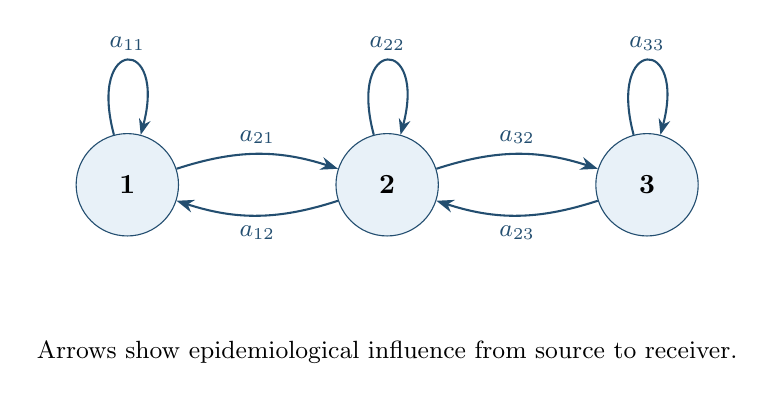
\begin{tikzpicture}[
  city/.style={circle,draw=deepblue,fill=softblue,minimum size=13mm,font=\bfseries},
  inter/.style={-{Stealth[length=2.2mm]},line width=0.75pt,deepblue},
  intra/.style={-{Stealth[length=2mm]},line width=0.75pt,deepblue},
  lab/.style={font=\small,align=center}
]
\node[city] (c1) at (0,0) {1};
\node[city] (c2) at (3.3,0) {2};
\node[city] (c3) at (6.6,0) {3};

\draw[inter,bend left=18] (c1) to node[above,lab] {$a_{21}$} (c2);
\draw[inter,bend left=18] (c2) to node[below,lab] {$a_{12}$} (c1);
\draw[inter,bend left=18] (c2) to node[above,lab] {$a_{32}$} (c3);
\draw[inter,bend left=18] (c3) to node[below,lab] {$a_{23}$} (c2);

\draw[intra] (c1) edge[loop above,min distance=13mm] node[above,lab] {$a_{11}$} (c1);
\draw[intra] (c2) edge[loop above,min distance=13mm] node[above,lab] {$a_{22}$} (c2);
\draw[intra] (c3) edge[loop above,min distance=13mm] node[above,lab] {$a_{33}$} (c3);

\node[lab,below=12mm of c2] {Arrows show epidemiological influence from source to receiver.};
\end{tikzpicture}
\caption{Three-city mobility corridor with one diagonal transmission channel in each city.}
\label{fig:three_city_network}
\end{figure}

The incoming source sets are
\[
\Min(1)=\{1,2\},
\qquad
\Min(2)=\{1,2,3\},
\qquad
\Min(3)=\{2,3\}.
\]

\subsection{State and differential equations}

For each city $i$, let $S_i,E_i,I_i,R_i$ denote the susceptible, exposed,
infectious, and removed fractions. The state is ordered as
\[
x=\col
(S_1,S_2,S_3,E_1,E_2,E_3,I_1,I_2,I_3,R_1,R_2,R_3)
\in\R^{12}.
\]
The city-specific equations are
\[
\begin{aligned}
\dot S_1
&=-\beta S_1(a_{11}I_1+a_{12}I_2),
&
\dot E_1
&=\beta S_1(a_{11}I_1+a_{12}I_2)-\sigma E_1,\\
\dot S_2
&=-\beta S_2(a_{21}I_1+a_{22}I_2+a_{23}I_3),
&
\dot E_2
&=\beta S_2(a_{21}I_1+a_{22}I_2+a_{23}I_3)-\sigma E_2,\\
\dot S_3
&=-\beta S_3(a_{32}I_2+a_{33}I_3),
&
\dot E_3
&=\beta S_3(a_{32}I_2+a_{33}I_3)-\sigma E_3,
\end{aligned}
\]
with
\[
\dot I_i=\sigma E_i-\gamma I_i,
\qquad
\dot R_i=\gamma I_i,
\qquad i=1,2,3.
\]

\subsection{Exact quadratic representation}

Define the seven infection products in the fixed channel order:
\[
\phi^{SI}(x)=\col(
S_1I_1,S_1I_2,
S_2I_1,S_2I_2,S_2I_3,
S_3I_2,S_3I_3).
\]
Let
\[
B_0=
\begin{bmatrix}
 a_{11} & a_{12} & 0 & 0 & 0 & 0 & 0\\
 0 & 0 & a_{21} & a_{22} & a_{23} & 0 & 0\\
 0 & 0 & 0 & 0 & 0 & a_{32} & a_{33}
\end{bmatrix}.
\]
Then the quadratic transmission contribution is represented by
\[
f_{\mathrm Q}(x)
=
\beta
\begin{bmatrix}
-B_0\\
 B_0\\
 0_{3\times7}\\
 0_{3\times7}
\end{bmatrix}
\phi^{SI}(x).
\]
The remaining compartmental transitions form a linear field
\[
f_{\mathrm L}(x)=A_{\ell}x.
\]
Thus the complete vector field is decomposed as
\[
f(x)=f_{\mathrm L}(x)+f_{\mathrm Q}(x).
\]
This decomposition is not merely notational. It separates the two operations
used by Algorithm~1:

\begin{itemize}[leftmargin=2em]
\item $f_{\mathrm Q}$ increases polynomial degree by one;
\item $f_{\mathrm L}$ preserves degree and therefore determines the linear
      closure required within each homogeneous block.
\end{itemize}

\section{Algorithm 1 in the present example}
\label{sec:algorithm}

For a homogeneous polynomial $q$ of degree $k$,
\[
\deg(\LieL q)=k,
\qquad
\deg(\LieQ q)=k+1.
\]
Accordingly, each homogeneous dictionary is constructed in two stages:

\[
\boxed{
\text{quadratic generation of degree }k+1
\quad\longrightarrow\quad
\text{linear closure within degree }k+1.
}
\]

For a set $\mathcal Q$ of degree-$k$ commutative monomials, define its linear
closure $\ClL(\mathcal Q)$ as the smallest degree-$k$ set containing
$\mathcal Q$ and all monomials generated by repeated application of
$\LieL$. In this SEIR model, linear closure replaces infectious factors by
exposed factors with the same city index, while preserving total degree and all
node indices.

\begin{flushleft}
\refstepcounter{algorithm}\label{alg:three_city_algorithm}%
\begin{tabularx}{\textwidth}{@{}>{\raggedleft\arraybackslash}p{0.06\textwidth}X@{}}
\toprule
\multicolumn{2}{@{}l@{}}{\textbf{Algorithm \thealgorithm} (Linearly closed graph-induced lifting for the three-city model)}\\
\midrule
1 & Decompose the vector field into $f=f_{\mathrm L}+f_{\mathrm Q}$.\\
2 & Create one quadratic transmission seed $S_iI_j$ for every channel $(i,j)\in\mathcalE$.\\
3 & Apply linear closure to the quadratic seeds. This adds $S_iE_j$ for every retained $S_iI_j$.\\
4 & Differentiate every degree-$k$ coordinate with $f_{\mathrm Q}$ and collect all distinct degree-$(k+1)$ monomials.\\
5 & Canonicalize products as commutative monomials, retain repeated factors, and merge duplicates. Coefficients are combined only within the same scalar derivative equation.\\
6 & Apply iterative linear closure to the new seed set until no same-degree monomial is missing.\\
7 & Choose a deterministic ordering, build the observable vector, and assemble the retained block operator.\\
8 & Verify linear closure. At truncation order $d$, place only the degree-$(d+1)$ terms generated by $f_{\mathrm Q}$ from the top retained block in the residual.\\
\bottomrule
\end{tabularx}
\end{flushleft}

The remainder of the document applies these steps explicitly up to degree
three and then performs a forward check at degree four.

\stepbox{Reading guide}{
The symbols with a hat, such as $\seedM_3^{\mathcalE}$, denote the seed set
created by the quadratic field. The unhatted set $\mathcal M_3^{\mathcalE}$
denotes the final linearly closed dictionary. This distinction is essential:
the seed set records where the nonlinear transmission mechanism first creates
new monomials, while the closure set records every same-degree coordinate
needed for exact propagation under the linear SEIR transitions.}

\section{Degree two: transmission seeds and linear closure}
\label{sec:degree_two}

\subsection{Mechanistic seed set}

Algorithm~1 begins with one susceptible--infectious product for each effective
transmission channel:
\[
\seedM_2^{\mathcalE}
=
\{
S_1I_1,S_1I_2,
S_2I_1,S_2I_2,S_2I_3,
S_3I_2,S_3I_3
\}.
\]
There are exactly seven seeds because there are seven channels. Each monomial
has an immediate epidemiological interpretation: $S_iI_j$ couples susceptible
individuals in receiving city $i$ with infectious individuals associated with
source city $j$.

\subsection{Why exposure observables appear}

The linear SEIR field acts on the factors as
\[
\dot S_i\big|_{f_{\mathrm L}}=0,
\qquad
\dot E_i\big|_{f_{\mathrm L}}=-\sigma E_i,
\qquad
\dot I_i\big|_{f_{\mathrm L}}=\sigma E_i-\gamma I_i.
\]
Hence
\[
\LieL(S_iI_j)
=
-\gamma S_iI_j+\sigma S_iE_j,
\]
whereas
\[
\LieL(S_iE_j)=-\sigma S_iE_j.
\]
The first derivative creates $S_iE_j$ from $S_iI_j$, and the second derivative
creates no further monomial. Therefore the closure terminates after one
expansion:
\[
\mathcal M_2^{\mathcalE}
=
\ClL(\seedM_2^{\mathcalE})
=
\{S_iI_j,S_iE_j:(i,j)\in\mathcalE\}.
\]
Explicitly,
\[
\begin{aligned}
\phi^{SI}(x)
={}&\col(
S_1I_1,S_1I_2,
S_2I_1,S_2I_2,S_2I_3,
S_3I_2,S_3I_3),\\
\phi^{SE}(x)
={}&\col(
S_1E_1,S_1E_2,
S_2E_1,S_2E_2,S_2E_3,
S_3E_2,S_3E_3).
\end{aligned}
\]
Thus
\[
\Phi_2^{\mathcalE}(x)=\col(\phi^{SI}(x),\phi^{SE}(x))\in\R^{14},
\]
and
\[
z_2^{\mathcalE}(x)=\col(x,\Phi_2^{\mathcalE}(x))\in\R^{26}.
\]

\stepbox{Conceptual point}{
The seven exposure products are not appended as an arbitrary enrichment. They
are forced by the linear transition from exposed to infectious compartments.
The first graph-induced dictionary is therefore the linear closure of the
mechanistic transmission seeds.}

\subsection{Comparison with complete quadratic coordinates}

The original state has 12 coordinates. A complete ordered quadratic tensor
would contain $12^2=144$ quadratic coordinates, giving 156 coordinates through
degree two. A complete symmetric quadratic basis contains
$\binom{13}{2}=78$ degree-two monomials, giving 90 coordinates through degree
two. The graph-induced construction retains only 14 quadratic observables and
therefore gives a 26-dimensional state.

\section{Degree-three seed generation by the quadratic field}
\label{sec:cubic_generation}

The degree-three seed set is generated from the complete quadratic dictionary:
\[
\seedM_3^{\mathcalE}
=
\bigcup_{q\in\mathcal M_2^{\mathcalE}}
\Mon_3(\LieQ q).
\]
Only the quadratic transmission field is used in this step. The linear field
has already been assigned a different role: it closes the homogeneous block
after the seeds have been created.

\subsection{Two general differentiation formulas}

For an infection observable $S_iI_j$, the quadratic field acts only through the
susceptible factor, because $f_{\mathrm Q}$ has zero infectious component:
\[
\LieQ(S_iI_j)
=
-\beta\sum_{\ell\in\Min(i)}
 a_{i\ell}S_iI_\ell I_j.
\]
This creates monomials of family $SII$.

For an exposure observable $S_iE_j$, the product rule has two contributions:
\[
\LieQ(S_iE_j)
=
(\dot S_i|_{f_{\mathrm Q}})E_j
+
S_i(\dot E_j|_{f_{\mathrm Q}}).
\]
Therefore
\[
\LieQ(S_iE_j)
=
-\beta\sum_{\ell\in\Min(i)}
 a_{i\ell}S_iI_\ell E_j
+
\beta\sum_{\ell\in\Min(j)}
 a_{j\ell}S_iS_jI_\ell.
\]
The first sum creates $SIE$ monomials. The second creates $SSI$ monomials.

\subsection{How the terms arise: representative calculations}

Consider the diagonal observable $S_1I_1$. Since city 1 receives infection
from cities 1 and 2,
\[
\begin{aligned}
\LieQ(S_1I_1)
&=(\dot S_1|_{f_{\mathrm Q}})I_1\\
&=-\beta S_1(a_{11}I_1+a_{12}I_2)I_1\\
&=-\beta a_{11}S_1I_1^2
  -\beta a_{12}S_1I_1I_2.
\end{aligned}
\]
The repeated factor $I_1^2$ is retained. It is a genuine commutative monomial,
not a duplicate to be removed.

For the off-diagonal observable $S_1I_2$,
\[
\LieQ(S_1I_2)
=-\beta a_{11}S_1I_1I_2
 -\beta a_{12}S_1I_2^2.
\]
The monomial $S_1I_1I_2$ also appeared in the preceding derivative. It will be
represented by one cubic dictionary coordinate, but it will occur in two
different rows of the degree-two-to-degree-three coupling matrix.

Now consider the diagonal exposure observable $S_1E_1$:
\[
\begin{aligned}
\LieQ(S_1E_1)
={}&-\beta S_1(a_{11}I_1+a_{12}I_2)E_1\\
&+\beta S_1^2(a_{11}I_1+a_{12}I_2)\\
={}&-\beta a_{11}S_1E_1I_1
   -\beta a_{12}S_1E_1I_2\\
&+\beta a_{11}S_1^2I_1
   +\beta a_{12}S_1^2I_2.
\end{aligned}
\]
The negative contribution comes from differentiating the susceptible factor;
the positive contribution comes from differentiating the exposed factor.

Finally, for the off-diagonal observable $S_1E_2$,
\[
\begin{aligned}
\LieQ(S_1E_2)
={}&-\beta S_1(a_{11}I_1+a_{12}I_2)E_2\\
&+\beta S_1S_2(a_{21}I_1+a_{22}I_2+a_{23}I_3).
\end{aligned}
\]
Thus it generates two $SIE$ terms and three $SSI$ terms. The second group
contains information from the incoming sources of city 2 because the exposed
factor belongs to city 2.

\subsection{Complete generation table}

The following table lists the distinct cubic terms generated in each scalar
quadratic-observable equation. Coefficients are omitted from the table only to
make dictionary membership easier to read; the complete coefficient-bearing
formulas are given in \cref{app:full_derivatives}.

% Generated by scripts/generate_example_artifacts.py
\begin{longtable}{@{}>{\raggedright\arraybackslash}p{0.17\textwidth}>{\raggedright\arraybackslash}p{0.76\textwidth}@{}}
\caption{Degree-three monomials generated by $f_{\mathrm Q}$ from each quadratic coordinate.}
\label{tab:cubic_generation}\\
\toprule
Quadratic coordinate & Distinct cubic monomials in $\LieQ q$\\
\midrule
\endfirsthead
\toprule
Quadratic coordinate & Distinct cubic monomials in $\LieQ q$\\
\midrule
\endhead
$S_1I_1$ & $S_1I_1^{2}$,\ $S_1I_1I_2$ \\
$S_1I_2$ & $S_1I_1I_2$,\ $S_1I_2^{2}$ \\
$S_2I_1$ & $S_2I_1^{2}$,\ $S_2I_1I_2$,\ $S_2I_1I_3$ \\
$S_2I_2$ & $S_2I_1I_2$,\ $S_2I_2^{2}$,\ $S_2I_2I_3$ \\
$S_2I_3$ & $S_2I_1I_3$,\ $S_2I_2I_3$,\ $S_2I_3^{2}$ \\
$S_3I_2$ & $S_3I_2^{2}$,\ $S_3I_2I_3$ \\
$S_3I_3$ & $S_3I_2I_3$,\ $S_3I_3^{2}$ \\
$S_1E_1$ & $S_1E_1I_1$,\ $S_1E_1I_2$,\ $S_1^{2}I_1$,\ $S_1^{2}I_2$ \\
$S_1E_2$ & $S_1E_2I_1$,\ $S_1E_2I_2$,\ $S_1S_2I_1$,\ $S_1S_2I_2$,\ $S_1S_2I_3$ \\
$S_2E_1$ & $S_2E_1I_1$,\ $S_2E_1I_2$,\ $S_2E_1I_3$,\ $S_1S_2I_1$,\ $S_1S_2I_2$ \\
$S_2E_2$ & $S_2E_2I_1$,\ $S_2E_2I_2$,\ $S_2E_2I_3$,\ $S_2^{2}I_1$,\ $S_2^{2}I_2$,\ $S_2^{2}I_3$ \\
$S_2E_3$ & $S_2E_3I_1$,\ $S_2E_3I_2$,\ $S_2E_3I_3$,\ $S_2S_3I_2$,\ $S_2S_3I_3$ \\
$S_3E_2$ & $S_3E_2I_2$,\ $S_3E_2I_3$,\ $S_2S_3I_1$,\ $S_2S_3I_2$,\ $S_2S_3I_3$ \\
$S_3E_3$ & $S_3E_3I_2$,\ $S_3E_3I_3$,\ $S_3^{2}I_2$,\ $S_3^{2}I_3$ \\
\bottomrule
\end{longtable}


Across the 14 scalar derivatives there are \NumRawCubic{} monomial appearances.
Before the final seed set is formed, all products are written in a canonical
commutative form.

\section{Commutative canonicalization and duplicate handling}
\label{sec:canonicalization}

\subsection{What canonicalization means}

The tensor representation is ordered, but the scalar observables are ordinary
commutative monomials. Consequently,
\[
S_1I_1I_2=S_1I_2I_1.
\]
The two products correspond to the same scalar observable and must occupy one
coordinate in the dictionary. By contrast,
\[
S_1I_1^2
\]
contains a repeated factor and remains a distinct monomial.

A practical canonical representation stores the exponent of every scalar
variable in a fixed order. For example, with the variable order
\[
S_1,S_2,S_3,E_1,E_2,E_3,I_1,I_2,I_3,
\]
the monomial $S_1I_1I_2$ is represented by the exponent vector
\[
(1,0,0,0,0,0,1,1,0).
\]
This representation is insensitive to factor order and preserves repeated
factors exactly.

\subsection{Two distinct notions of duplication}

It is important to distinguish two cases.

\begin{enumerate}[leftmargin=2em]
\item \textbf{Duplicate terms within one scalar derivative.} If the same
      canonical monomial is produced more than once in one derivative equation,
      its coefficients must be added before the operator row is assembled.
\item \textbf{The same coordinate generated in different scalar derivatives.}
      The dictionary still contains one coordinate, but each derivative has its
      own matrix entry in the column associated with that coordinate.
\end{enumerate}

In the present degree-two-to-degree-three calculation, no exact within-row
duplicate or cancellation remains when the channel weights are retained
symbolically. Nine cubic coordinates are, however, shared by two different
scalar derivative equations:

% Generated by scripts/generate_example_artifacts.py
\begin{center}
\begin{tabular}{@{}p{0.25\textwidth}p{0.65\textwidth}@{}}
\toprule
Shared cubic coordinate & Generating scalar derivatives\\
\midrule
$S_1I_1I_2$ & $\LieQ(S_1I_1)$ and $\LieQ(S_1I_2)$ \\
$S_2I_1I_2$ & $\LieQ(S_2I_2)$ and $\LieQ(S_2I_1)$ \\
$S_2I_1I_3$ & $\LieQ(S_2I_3)$ and $\LieQ(S_2I_1)$ \\
$S_2I_2I_3$ & $\LieQ(S_2I_2)$ and $\LieQ(S_2I_3)$ \\
$S_3I_2I_3$ & $\LieQ(S_3I_3)$ and $\LieQ(S_3I_2)$ \\
$S_1S_2I_1$ & $\LieQ(S_1E_2)$ and $\LieQ(S_2E_1)$ \\
$S_1S_2I_2$ & $\LieQ(S_1E_2)$ and $\LieQ(S_2E_1)$ \\
$S_2S_3I_2$ & $\LieQ(S_2E_3)$ and $\LieQ(S_3E_2)$ \\
$S_2S_3I_3$ & $\LieQ(S_2E_3)$ and $\LieQ(S_3E_2)$ \\
\bottomrule
\end{tabular}
\end{center}


For example, the column associated with $S_1I_1I_2$ contains
\[
-\beta a_{12}
\]
in the row for $\frac{d}{dt}(S_1I_1)$ and
\[
-\beta a_{11}
\]
in the row for $\frac{d}{dt}(S_1I_2)$. These coefficients are not added
together because they belong to different equations.

After merging the nine repeated coordinates across different rows, the
\NumRawCubic{} appearances reduce to
\[
\NumRawCubic-9=\NumMthreeSeeds
\]
distinct cubic seeds. They are distributed as follows:
\[
12\text{ of type }SII,
\qquad
17\text{ of type }SIE,
\qquad
13\text{ of type }SSI.
\]
Thus
\[
|\seedM_3^{\mathcalE}|=\NumMthreeSeeds.
\]

\stepbox{Why the seed count is not yet the final cubic dimension}{
The 42 seeds are all cubic coordinates created directly by the nonlinear
transmission mechanism. They need not form an invariant degree-three block
under the linear SEIR transitions. Algorithm~1 therefore applies linear
closure before defining the final cubic dictionary.}

\section{Linear closure of the cubic seed set}
\label{sec:linear_closure}

The final cubic dictionary is
\[
\mathcal M_3^{\mathcalE}
=
\ClL(\seedM_3^{\mathcalE}).
\]
This section shows explicitly what the closure operation adds and why it
terminates.

\subsection{General action of the linear SEIR field}

Let $q$ be a monomial that contains $b_i$ copies of $E_i$ and $c_i$ copies of
$I_i$. Since $S_i$ is constant under $f_{\mathrm L}$, the product rule gives
\[
\LieL q
=
-\left(\sigma\sum_i b_i+\gamma\sum_i c_i\right)q
+
\sigma\sum_{i:c_i>0}
 c_i\,q\frac{E_i}{I_i}.
\]
The notation $qE_i/I_i$ means that one factor $I_i$ is replaced by $E_i$.
The coefficient $c_i$ records the number of identical infectious factors that
can be differentiated. Thus, for example,
\[
\LieL(S_1I_1^2)
=-2\gamma S_1I_1^2+2\sigma S_1E_1I_1.
\]
Applying the linear derivative again generates $S_1E_1^2$. No new node index
and no new polynomial degree is introduced.

\subsection{Closure chains by monomial family}

The cubic seeds belong to three families. Their closure chains are:

\begin{align*}
SII
&\longrightarrow SIE\longrightarrow SEE,\\
SIE
&\longrightarrow SEE,\\
SSI
&\longrightarrow SSE.
\end{align*}

For example,
\[
S_1I_1I_2
\longrightarrow
\{S_1E_1I_2,\ S_1I_1E_2\}
\longrightarrow
S_1E_1E_2.
\]
Similarly,
\[
S_1S_2I_3\longrightarrow S_1S_2E_3.
\]
The intermediate $SIE$ variants generated from the $SII$ seeds are already
present among the 17 cubic seeds generated directly from the quadratic
exposure observables. Consequently, the only new family types added by closure
in this example are $SEE$ and $SSE$.

\subsection{Coordinates added by closure}

The 12 new $SEE$ monomials are
\[
\begin{aligned}
\{&S_1E_1^2,S_1E_1E_2,S_1E_2^2,\\
  &S_2E_1^2,S_2E_1E_2,S_2E_1E_3,
   S_2E_2^2,S_2E_2E_3,S_2E_3^2,\\
  &S_3E_2^2,S_3E_2E_3,S_3E_3^2\}.
\end{aligned}
\]
The 13 new $SSE$ monomials are
\[
\begin{aligned}
\{&S_1^2E_1,S_1^2E_2,\\
  &S_1S_2E_1,S_1S_2E_2,S_1S_2E_3,\\
  &S_2^2E_1,S_2^2E_2,S_2^2E_3,\\
  &S_2S_3E_1,S_2S_3E_2,S_2S_3E_3,\\
  &S_3^2E_2,S_3^2E_3\}.
\end{aligned}
\]
The family counts are therefore:

% Generated by scripts/generate_example_artifacts.py
\begin{center}
\begin{tabular}{@{}lrrr@{}}
\toprule
Family & Quadratic seeds & Added by closure & Final count\\
\midrule
$SII$ & 12 & 0 & 12 \\
$SIE$ & 17 & 0 & 17 \\
$SEE$ & 0 & 12 & 12 \\
$SSI$ & 13 & 0 & 13 \\
$SSE$ & 0 & 13 & 13 \\
\midrule
Total & 42 & 25 & 67 \\
\bottomrule
\end{tabular}
\end{center}


Hence
\[
|\mathcal M_3^{\mathcalE}|
=
\NumMthreeSeeds+\NumMthreeClosure
=
\NumMthree.
\]

\subsection{Direct closure checks}

Two representative checks are
\[
\LieL(S_1I_1E_1)
=
\sigma S_1E_1^2-(\gamma+\sigma)S_1I_1E_1,
\]
and
\[
\LieL(S_1^2I_1)
=
\sigma S_1^2E_1-\gamma S_1^2I_1.
\]
The newly produced monomials $S_1E_1^2$ and $S_1^2E_1$ are both included in
$\mathcal M_3^{\mathcalE}$.

The accompanying verification script checks the stronger statement
\[
\Mon_3(\LieL q)\subseteq\mathcal M_3^{\mathcalE}
\qquad
\text{for every }q\in\mathcal M_3^{\mathcalE}.
\]
Therefore no degree-three term is omitted when the cubic block is
differentiated.

\section{Assembly of the lifted systems}
\label{sec:lifted_system}

\subsection{First closure}

The first lifted state is
\[
z_2^{\mathcalE}(x)
=
\col(x,\Phi_2^{\mathcalE}(x))
\in\R^{26}.
\]
The original state equations are exactly linear in $x$ and the infection block
of $\Phi_2^{\mathcalE}$. Differentiating the quadratic observables gives terms
retained in $\Phi_2^{\mathcalE}$ plus cubic terms. Thus
\[
\dot z_2^{\mathcalE}
=
\matK_2^{\mathcalE}z_2^{\mathcalE}
+r_2^{\mathcalE}(x),
\]
where the first 12 residual components are zero. For a channel
$(i,j)\in\mathcalE$, the two nonzero residual blocks have components
\[
(r_{SI}^{\mathcalE})_{(i,j)}
=
-\beta\sum_{\ell\in\Min(i)}
 a_{i\ell}S_iI_\ell I_j,
\]
\[
(r_{SE}^{\mathcalE})_{(i,j)}
=
-\beta\sum_{\ell\in\Min(i)}
 a_{i\ell}S_iI_\ell E_j
+
\beta\sum_{\ell\in\Min(j)}
 a_{j\ell}S_iS_jI_\ell.
\]
The 42 cubic seeds identified in \cref{sec:cubic_generation} are precisely the
distinct monomials appearing in these residual components.

\subsection{Order-three state}

Choose the deterministic ordering in \cref{app:dictionary} and define
\[
\Phi_3^{\mathcalE}(x)
=
[q(x)]_{q\in\mathcal M_3^{\mathcalE}}
\in\R^{67}.
\]
The order-three lifted state is
\[
z_3^{\mathcalE}(x)
=
\col(x,\Phi_2^{\mathcalE}(x),\Phi_3^{\mathcalE}(x))
\in\R^{93}.
\]
Its dimension is
\[
\dim z_3^{\mathcalE}
=12+14+67
=93.
\]

The exact infinite hierarchy has the degree-block structure
\[
\begin{aligned}
\dot x
&=\matK_{1,1}x+\matK_{1,2}\Phi_2^{\mathcalE},\\
\dot\Phi_2^{\mathcalE}
&=\matK_{2,2}\Phi_2^{\mathcalE}
 +\matK_{2,3}\Phi_3^{\mathcalE},\\
\dot\Phi_3^{\mathcalE}
&=\matK_{3,3}\Phi_3^{\mathcalE}
 +\matK_{3,4}\Phi_4^{\mathcalE}.
\end{aligned}
\]
The relevant retained block sizes are
\[
\matK_{1,1}\in\R^{12\times12},
\quad
\matK_{1,2}\in\R^{12\times14},
\]
\[
\matK_{2,2}\in\R^{14\times14},
\quad
\matK_{2,3}\in\R^{14\times67},
\quad
\matK_{3,3}\in\R^{67\times67}.
\]

At order three, the quartic block is not retained. Therefore
\[
\dot z_3^{\mathcalE}
=
\matK_3^{\mathcalE}z_3^{\mathcalE}
+r_3^{\mathcalE}(x),
\]
with
\[
r_3^{\mathcalE}(x)
=
\col\bigl(0_{12},0_{14},\LieQ\Phi_3^{\mathcalE}(x)\bigr).
\]
Every nonzero residual component is homogeneous of degree four. No omitted
cubic term remains because $\mathcal M_3^{\mathcalE}$ is linearly closed.

\subsection{Comparison with complete degree-three liftings}

A complete ordered lifting through degree three would contain
\[
12+12^2+12^3=1884
\]
coordinates. A complete symmetric monomial lifting through degree three would
contain
\[
12+\binom{13}{2}+\binom{14}{3}
=12+78+364
=454
\]
coordinates. The graph-induced linearly closed construction contains 93.
This comparison is finite-dimensional and illustrative; it does not assert
minimality or optimality of the graph-induced dictionary.

\section{Forward consistency check at degree four}
\label{sec:forward_check}

The order-three construction can be checked by applying the same two-stage
rule once more. The quadratic field acts on all 67 cubic coordinates and
generates
\[
|\seedM_4^{\mathcalE}|=\NumMfourSeeds
\]
distinct quartic seeds. Iterative linear closure expands this set to
\[
|\mathcal M_4^{\mathcalE}|=\NumMfour.
\]

These quartic values are not needed to define $z_3^{\mathcalE}$, but they
serve two purposes:

\begin{enumerate}[leftmargin=2em]
\item They verify that the recursion is not a special correction applied only
      at degree three.
\item They confirm that the order-three residual is exactly the forcing that
      initiates the degree-four seed set.
\end{enumerate}

The closure check also confirms
\[
\Mon_4(\LieL q)\subseteq\mathcal M_4^{\mathcalE}
\qquad
\text{for every }q\in\mathcal M_4^{\mathcalE}.
\]
Thus the same architecture continues:
\[
\text{closed degree 3}
\xrightarrow{\ f_{\mathrm Q}\ }
\text{degree-4 seeds}
\xrightarrow{\ f_{\mathrm L}\ }
\text{closed degree 4}.
\]

\section{Interpretation of the generated nonlinear terms}
\label{sec:interpretation}

The worked example makes the origin of each monomial family transparent.

\subsection{The SII family}

A term $S_iI_\ell I_j$ appears when the susceptible factor in the infection
observable $S_iI_j$ is differentiated. One infectious factor, $I_j$, was
already present in the observable; the second, $I_\ell$, comes from an incoming
source of city $i$. These terms therefore encode pairs of infectious factors
sharing the same receiving susceptible population.

\subsection{The SIE and SEE families}

A term $S_iI_\ell E_j$ appears when the susceptible factor in $S_iE_j$ is
differentiated. Linear closure then replaces infectious factors by their
exposed counterparts and produces $SEE$ coordinates. These coordinates are
required because exposed and infectious variables are coupled by the linear
compartmental progression.

\subsection{The SSI and SSE families}

A term $S_iS_jI_\ell$ appears when the exposed factor in $S_iE_j$ is
differentiated through the positive transmission contribution to $\dot E_j$.
It links the susceptible factor already present at receiving city $i$ to the
susceptible population and incoming infectious source structure of city $j$.
Linear closure converts the infectious factor into an exposed factor and adds
the corresponding $SSE$ coordinate.

\subsection{Effect of diagonal channels}

Diagonal channels create terms such as
\[
S_iI_i^2,
\qquad
S_iE_iI_i,
\qquad
S_i^2I_i,
\]
and their linearly closed variants. These are not algebraic anomalies. They
represent aggregate within-city transmission and naturally contain repeated
city indices and repeated scalar factors.

\subsection{What the example does and does not establish}

The example establishes the exact operation of Algorithm~1 on a concrete
network and verifies the reported dictionary dimensions. It illustrates how
network support controls which polynomial interactions are generated. It does
not claim that the resulting dictionary is the smallest possible invariant or
approximately invariant dictionary, nor does it provide a trajectory-error
bound for a finite truncation.

\section{Summary of the complete construction}
\label{sec:summary}

Applying Algorithm~1 to the three-city model gives the following sequence:

\begin{enumerate}[leftmargin=2em,label=\arabic*.]
\item Seven effective transmission channels produce seven quadratic
      susceptible--infectious seeds.
\item Linear closure adds seven susceptible--exposed coordinates, giving
      $|\mathcal M_2^{\mathcalE}|=14$ and $\dim z_2^{\mathcalE}=26$.
\item The quadratic field produces 51 cubic appearances across the 14 scalar
      derivative equations.
\item Commutative canonicalization merges nine coordinates shared by different
      equations, leaving 42 distinct cubic seeds.
\item Linear closure adds 12 $SEE$ and 13 $SSE$ monomials. The final cubic
      dictionary contains 67 coordinates.
\item The order-three lifted state contains $12+14+67=93$ coordinates.
\item The cubic dictionary is closed under the linear SEIR field, so the
      order-three residual contains only quartic terms.
\item A forward application of the same algorithm generates 159 quartic seeds
      and a 223-element linearly closed quartic dictionary.
\end{enumerate}

The key distinction is therefore
\[
\boxed{
42\text{ cubic transmission seeds}
\quad\neq\quad
67\text{ coordinates in the final cubic dictionary}.
}
\]
The difference consists precisely of the same-degree coordinates required by
linear compartmental closure.

All counts in this document are regenerated and checked by the accompanying
standard-library Python script. The generated CSV and TeX tables provide an
auditable link between the mathematical derivation and the machine
verification.


\appendix
\section{Complete derivatives of the 14 quadratic observables}
\label{app:full_derivatives}

This appendix retains every coefficient and separates no terms. It provides a
row-by-row source for the blocks $\matK_{2,2}$ and $\matK_{2,3}$.

\subsection{Susceptible--infectious observables}

\begin{align*}
\frac{d}{dt}(S_1I_1)
={}&-\gamma S_1I_1+\sigma S_1E_1
-\beta a_{11}S_1I_1^2
-\beta a_{12}S_1I_1I_2,\\
\frac{d}{dt}(S_1I_2)
={}&-\gamma S_1I_2+\sigma S_1E_2
-\beta a_{11}S_1I_1I_2
-\beta a_{12}S_1I_2^2,\\
\frac{d}{dt}(S_2I_1)
={}&-\gamma S_2I_1+\sigma S_2E_1
-\beta a_{21}S_2I_1^2
-\beta a_{22}S_2I_1I_2
-\beta a_{23}S_2I_1I_3,\\
\frac{d}{dt}(S_2I_2)
={}&-\gamma S_2I_2+\sigma S_2E_2
-\beta a_{21}S_2I_1I_2
-\beta a_{22}S_2I_2^2
-\beta a_{23}S_2I_2I_3,\\
\frac{d}{dt}(S_2I_3)
={}&-\gamma S_2I_3+\sigma S_2E_3
-\beta a_{21}S_2I_1I_3
-\beta a_{22}S_2I_2I_3
-\beta a_{23}S_2I_3^2,\\
\frac{d}{dt}(S_3I_2)
={}&-\gamma S_3I_2+\sigma S_3E_2
-\beta a_{32}S_3I_2^2
-\beta a_{33}S_3I_2I_3,\\
\frac{d}{dt}(S_3I_3)
={}&-\gamma S_3I_3+\sigma S_3E_3
-\beta a_{32}S_3I_2I_3
-\beta a_{33}S_3I_3^2.
\end{align*}

\subsection{Susceptible--exposed observables}

\begin{align*}
\frac{d}{dt}(S_1E_1)
={}&-\sigma S_1E_1
-\beta a_{11}S_1I_1E_1
-\beta a_{12}S_1I_2E_1
+\beta a_{11}S_1^2I_1
+\beta a_{12}S_1^2I_2,\\
\frac{d}{dt}(S_1E_2)
={}&-\sigma S_1E_2
-\beta a_{11}S_1I_1E_2
-\beta a_{12}S_1I_2E_2\\
&+\beta a_{21}S_1S_2I_1
+\beta a_{22}S_1S_2I_2
+\beta a_{23}S_1S_2I_3,\\
\frac{d}{dt}(S_2E_1)
={}&-\sigma S_2E_1
-\beta a_{21}S_2I_1E_1
-\beta a_{22}S_2I_2E_1
-\beta a_{23}S_2I_3E_1\\
&+\beta a_{11}S_1S_2I_1
+\beta a_{12}S_1S_2I_2,\\
\frac{d}{dt}(S_2E_2)
={}&-\sigma S_2E_2
-\beta a_{21}S_2I_1E_2
-\beta a_{22}S_2I_2E_2
-\beta a_{23}S_2I_3E_2\\
&+\beta a_{21}S_2^2I_1
+\beta a_{22}S_2^2I_2
+\beta a_{23}S_2^2I_3,\\
\frac{d}{dt}(S_2E_3)
={}&-\sigma S_2E_3
-\beta a_{21}S_2I_1E_3
-\beta a_{22}S_2I_2E_3
-\beta a_{23}S_2I_3E_3\\
&+\beta a_{32}S_2S_3I_2
+\beta a_{33}S_2S_3I_3,\\
\frac{d}{dt}(S_3E_2)
={}&-\sigma S_3E_2
-\beta a_{32}S_3I_2E_2
-\beta a_{33}S_3I_3E_2\\
&+\beta a_{21}S_2S_3I_1
+\beta a_{22}S_2S_3I_2
+\beta a_{23}S_2S_3I_3,\\
\frac{d}{dt}(S_3E_3)
={}&-\sigma S_3E_3
-\beta a_{32}S_3I_2E_3
-\beta a_{33}S_3I_3E_3
+\beta a_{32}S_3^2I_2
+\beta a_{33}S_3^2I_3.
\end{align*}

In each equation, the quadratic terms belong to $\mathcal M_2^{\mathcalE}$ and
form the degree-preserving block $\matK_{2,2}$. The cubic terms belong to the
42-element seed set $\seedM_3^{\mathcalE}$ and populate the block
$\matK_{2,3}$ after the final 67-coordinate cubic ordering has been fixed.

\section{Complete linearly closed cubic dictionary}
\label{app:dictionary}

The following deterministic ordering groups the monomials by family. The
``origin'' column distinguishes coordinates generated directly by the
quadratic transmission field from coordinates added by linear closure.

% Generated by scripts/generate_example_artifacts.py
\begin{longtable}{@{}rlll@{}}
\caption{Complete 67-element cubic dictionary $\mathcal M_3^{\mathcalE}$.}
\label{tab:complete_m3_dictionary}\\
\toprule
Index & Family & Monomial & Origin\\
\midrule
\endfirsthead
\toprule
Index & Family & Monomial & Origin\\
\midrule
\endhead
1 & SII & $S_1I_1^{2}$ & quadratic seed \\
2 & SII & $S_1I_1I_2$ & quadratic seed \\
3 & SII & $S_1I_2^{2}$ & quadratic seed \\
4 & SII & $S_2I_1^{2}$ & quadratic seed \\
5 & SII & $S_2I_1I_2$ & quadratic seed \\
6 & SII & $S_2I_1I_3$ & quadratic seed \\
7 & SII & $S_2I_2^{2}$ & quadratic seed \\
8 & SII & $S_2I_2I_3$ & quadratic seed \\
9 & SII & $S_2I_3^{2}$ & quadratic seed \\
10 & SII & $S_3I_2^{2}$ & quadratic seed \\
11 & SII & $S_3I_2I_3$ & quadratic seed \\
12 & SII & $S_3I_3^{2}$ & quadratic seed \\
13 & SIE & $S_1E_1I_1$ & quadratic seed \\
14 & SIE & $S_1E_1I_2$ & quadratic seed \\
15 & SIE & $S_1E_2I_1$ & quadratic seed \\
16 & SIE & $S_1E_2I_2$ & quadratic seed \\
17 & SIE & $S_2E_1I_1$ & quadratic seed \\
18 & SIE & $S_2E_1I_2$ & quadratic seed \\
19 & SIE & $S_2E_1I_3$ & quadratic seed \\
20 & SIE & $S_2E_2I_1$ & quadratic seed \\
21 & SIE & $S_2E_2I_2$ & quadratic seed \\
22 & SIE & $S_2E_2I_3$ & quadratic seed \\
23 & SIE & $S_2E_3I_1$ & quadratic seed \\
24 & SIE & $S_2E_3I_2$ & quadratic seed \\
25 & SIE & $S_2E_3I_3$ & quadratic seed \\
26 & SIE & $S_3E_2I_2$ & quadratic seed \\
27 & SIE & $S_3E_2I_3$ & quadratic seed \\
28 & SIE & $S_3E_3I_2$ & quadratic seed \\
29 & SIE & $S_3E_3I_3$ & quadratic seed \\
30 & SEE & $S_1E_1^{2}$ & linear closure \\
31 & SEE & $S_1E_1E_2$ & linear closure \\
32 & SEE & $S_1E_2^{2}$ & linear closure \\
33 & SEE & $S_2E_1^{2}$ & linear closure \\
34 & SEE & $S_2E_1E_2$ & linear closure \\
35 & SEE & $S_2E_1E_3$ & linear closure \\
36 & SEE & $S_2E_2^{2}$ & linear closure \\
37 & SEE & $S_2E_2E_3$ & linear closure \\
38 & SEE & $S_2E_3^{2}$ & linear closure \\
39 & SEE & $S_3E_2^{2}$ & linear closure \\
40 & SEE & $S_3E_2E_3$ & linear closure \\
41 & SEE & $S_3E_3^{2}$ & linear closure \\
42 & SSI & $S_1^{2}I_1$ & quadratic seed \\
43 & SSI & $S_1^{2}I_2$ & quadratic seed \\
44 & SSI & $S_1S_2I_1$ & quadratic seed \\
45 & SSI & $S_1S_2I_2$ & quadratic seed \\
46 & SSI & $S_1S_2I_3$ & quadratic seed \\
47 & SSI & $S_2^{2}I_1$ & quadratic seed \\
48 & SSI & $S_2^{2}I_2$ & quadratic seed \\
49 & SSI & $S_2^{2}I_3$ & quadratic seed \\
50 & SSI & $S_2S_3I_1$ & quadratic seed \\
51 & SSI & $S_2S_3I_2$ & quadratic seed \\
52 & SSI & $S_2S_3I_3$ & quadratic seed \\
53 & SSI & $S_3^{2}I_2$ & quadratic seed \\
54 & SSI & $S_3^{2}I_3$ & quadratic seed \\
55 & SSE & $S_1^{2}E_1$ & linear closure \\
56 & SSE & $S_1^{2}E_2$ & linear closure \\
57 & SSE & $S_1S_2E_1$ & linear closure \\
58 & SSE & $S_1S_2E_2$ & linear closure \\
59 & SSE & $S_1S_2E_3$ & linear closure \\
60 & SSE & $S_2^{2}E_1$ & linear closure \\
61 & SSE & $S_2^{2}E_2$ & linear closure \\
62 & SSE & $S_2^{2}E_3$ & linear closure \\
63 & SSE & $S_2S_3E_1$ & linear closure \\
64 & SSE & $S_2S_3E_2$ & linear closure \\
65 & SSE & $S_2S_3E_3$ & linear closure \\
66 & SSE & $S_3^{2}E_2$ & linear closure \\
67 & SSE & $S_3^{2}E_3$ & linear closure \\
\bottomrule
\end{longtable}


\section{Traceability and reproducibility map}
\label{app:traceability}

\small
\begin{longtable}{@{}p{0.12\textwidth}p{0.29\textwidth}p{0.51\textwidth}@{}}
\caption{Mapping from Algorithm~1 to this document and the machine-verification files.}\\
\toprule
Algorithm step & Mathematical location & Reproducibility artifact\\
\midrule
\endfirsthead
\toprule
Algorithm step & Mathematical location & Reproducibility artifact\\
\midrule
\endhead
1 & Vector-field split in \cref{sec:network} & Constants and rules in \path{scripts/generate_example_artifacts.py}\\
2 & Quadratic seeds in \cref{sec:degree_two} & Generated count \texttt{M2\_seed\_count}\\
3 & Quadratic linear closure in \cref{sec:degree_two} & Closure assertion for every degree-two coordinate\\
4 & Cubic generation in \cref{sec:cubic_generation} & \path{generated/cubic_generation_rows.tex}\\
5 & Canonicalization in \cref{sec:canonicalization} & Exponent-vector monomial representation and shared-coordinate CSV\\
6 & Cubic linear closure in \cref{sec:linear_closure} & Closure assertion and final dictionary CSV\\
7 & Lifted-state assembly in \cref{sec:lifted_system} & Counts in \path{data/three_city_dictionary_counts.csv}\\
8 & Degree-four forward check in \cref{sec:forward_check} & Automatic checks for 159 seeds and 223 closed monomials\\
\bottomrule
\end{longtable}
\normalsize

\subsection*{Regeneration command}

From the root of this example folder, run
\begin{verbatim}
python scripts/generate_example_artifacts.py
\end{verbatim}
The command regenerates the CSV files and all TeX table fragments under
\texttt{generated/}. It terminates with an assertion failure if any expected
count or closure property changes.

\subsection*{Document build}

Compile with
\begin{verbatim}
latexmk -pdf main.tex
\end{verbatim}
The generated files must be present before compilation. They are included in
the distributed archive, but they can always be regenerated from the script.


\end{document}
